% Chapter Template

\chapter{Software Architecture} % Main chapter title

\label{Chapter4} % Change X to a consecutive number; for referencing this chapter elsewhere, use \ref{ChapterX}

\lhead{Chapter 4. \emph{Software Architecture}} % Change X to a consecutive number; this is for the header on each page - perhaps a shortened title

\section{Introduction}
An overview of the software architecture for {\em PySchedCL} is depicted in Fig. \ref{fig:pyschedcl}. The framework consists of two distinct modules, the functionalities of which are elaborated as follows.
	\begin{figure}[ht]  
		\centering
		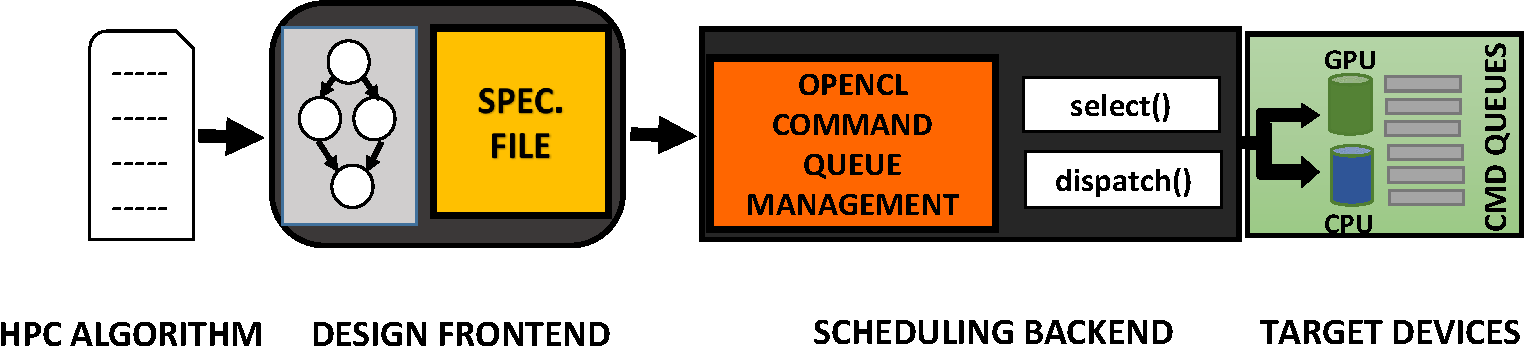
\includegraphics[scale=0.50]{Pictures/TCOverviewNonML.pdf}
		\caption{PySchedCL Toolflow\label{fig:pyschedcl}}
	\end{figure}
	\begin{enumerate}
		\item \textbf{Design Frontend: }The input to the scheduling framework is an OpenCL application represented in the form of a task graph $G$ as discussed earlier. The proposed framework supports a specification file using which programmers can easily design an OpenCL application for execution on a heterogeneous platform. The programmer requires to implement only the OpenCL kernels and provide configuration parameters  such as the dimensions of the input/output dataspace along with dependency information between kernels in this specification file.
		\item \textbf{Scheduling Backend: }The scheduling backend takes as input the specification file in Step 1, and schedules the computation of each data parallel kernel in the application across the devices of a heterogeneous CPU/GPU platform. This is achieved with the help of select and dispatch routines. The framework uses the {\tt select} function to i)choose a task component from $G$ and ii) select an available device (CPU/GPU). It next uses the {\tt dispatch} (line 8) routine for finally issuing relevant write, ndrange and read commands now specified in $\mathcal{Q}$ to target devices. The backend API also supports end designers to implement custom scheduling heuristics by overriding the functionalities of the {\tt select} and {\tt dispatch} routines.
		%In this communication, we highlight how popular scheduling heuristics such as standard list scheduling policies \cite{heft,zhao1,zhao2,hcpt,hps,pets,lookahead,plannerguide,owm,fdws} as well as standard cluster scheduling policies \cite{triplet,chp,rac,fcs,cmwsl} can be implemented. We also show how statistics obtained statically for a target application can be used along with the scheduling policies for designing intelligent scheduling heuristics. 
	\end{enumerate}
    The modular design of the scheduling backend is an integral feature of the framework. The default {\tt select} routine expects a static assignment of kernels to devices prior to the execution. It can be substituted by the user very easily with other scheduling policies which can even be dynamic in nature. The experimental section of this thesis extensively uses this modular feature of the {\tt select} function to implement and compare several scheduling policies on the transformer DAG. Additionally, experiments with a Machine Learning based scheduling policy have also been performed in a similar fashion. 
    \par We next elicit implementation details for each of the two modules  constituting the framework in the following subsections. 
    
    \section{Input File Specification}
	The specification file used in {\em PySchedCL} is written using the Javascript Object Notation (JSON) file format. The file consists of a collection of key value pairs depicting  necessary attribute information for an OpenCL kernel which includes information regarding input/output buffers, variables passed as arguments to the kernel call, the dimension of the kernel etc. Our tool processes this specification file and uses the scheduling backend to mimic the execution of a host program executing this kernel. 
	\par We have a LLVM compiler pass which parses the abstract syntax tree of an OpenCL kernel and generates an incomplete JSON file. The pass understands the dimensionality of the kernel, the types and positions of each variable and buffer used in the kernel function call. It also classifies buffers as input/output buffers by understanding whether it is treated as \textit{l-values} or \textit{r-values} in the body of the function. Given this file, the user is only required to specify guidance parameters which include 
	\begin{itemize}
		\item the size of the buffers
		\item the number of work items
		\item the values of the variable arguments
		\item the device and the number of command queues to be used
	\end{itemize}
	
	 The user has the option of either hardcoding constant numbers or writing expressions containing symbolic variables that depicts the relationship between work items and the dataspace to be processed. This ensures that we have one specification file for a kernel and the final values of these symbolic variables can be provided as command line parameters at runtime. We explain this by designing a JSON specification file for the matrix multiplication kernel depicted in Listing 1.

    \begin{lstlisting}[caption={OpenCL Kernel for Matrix Multiplication},captionpos=b,frame=single,basicstyle=\tiny,language=C]
        __kernel void gemm(__global float *A, __global float *B, __global float *C, 
        int M, int N, int K) {
        int ty = get_global_id(1);
        int tx = get_global_id(0);
        if ((tx < N) && (ty < M))
        {
        C[ty * N + tx] = 0;
        for(int k=0; k < K; k++)
        C[ty * N + tx] += A[ty * K + k] * B[k * N +tx];
        }
        
        }
    \end{lstlisting}

    The matrix multiplication kernel is a 2-D kernel which takes as input two matrices $A$, $B$ of dimensions $M \times K$, $K \times N$ respectively and produces an output matrix $C$ of dimension $M \times N$. A total of $M*N$ work items is launched where the job of each work item is computing the dot product of one row of $A$ and one column of $B$ to produce one element of $C$. The JSON specification file for the same is depicted in Fig. \ref{fig:json}
    
    \begin{figure}[ht]  
		\centering
		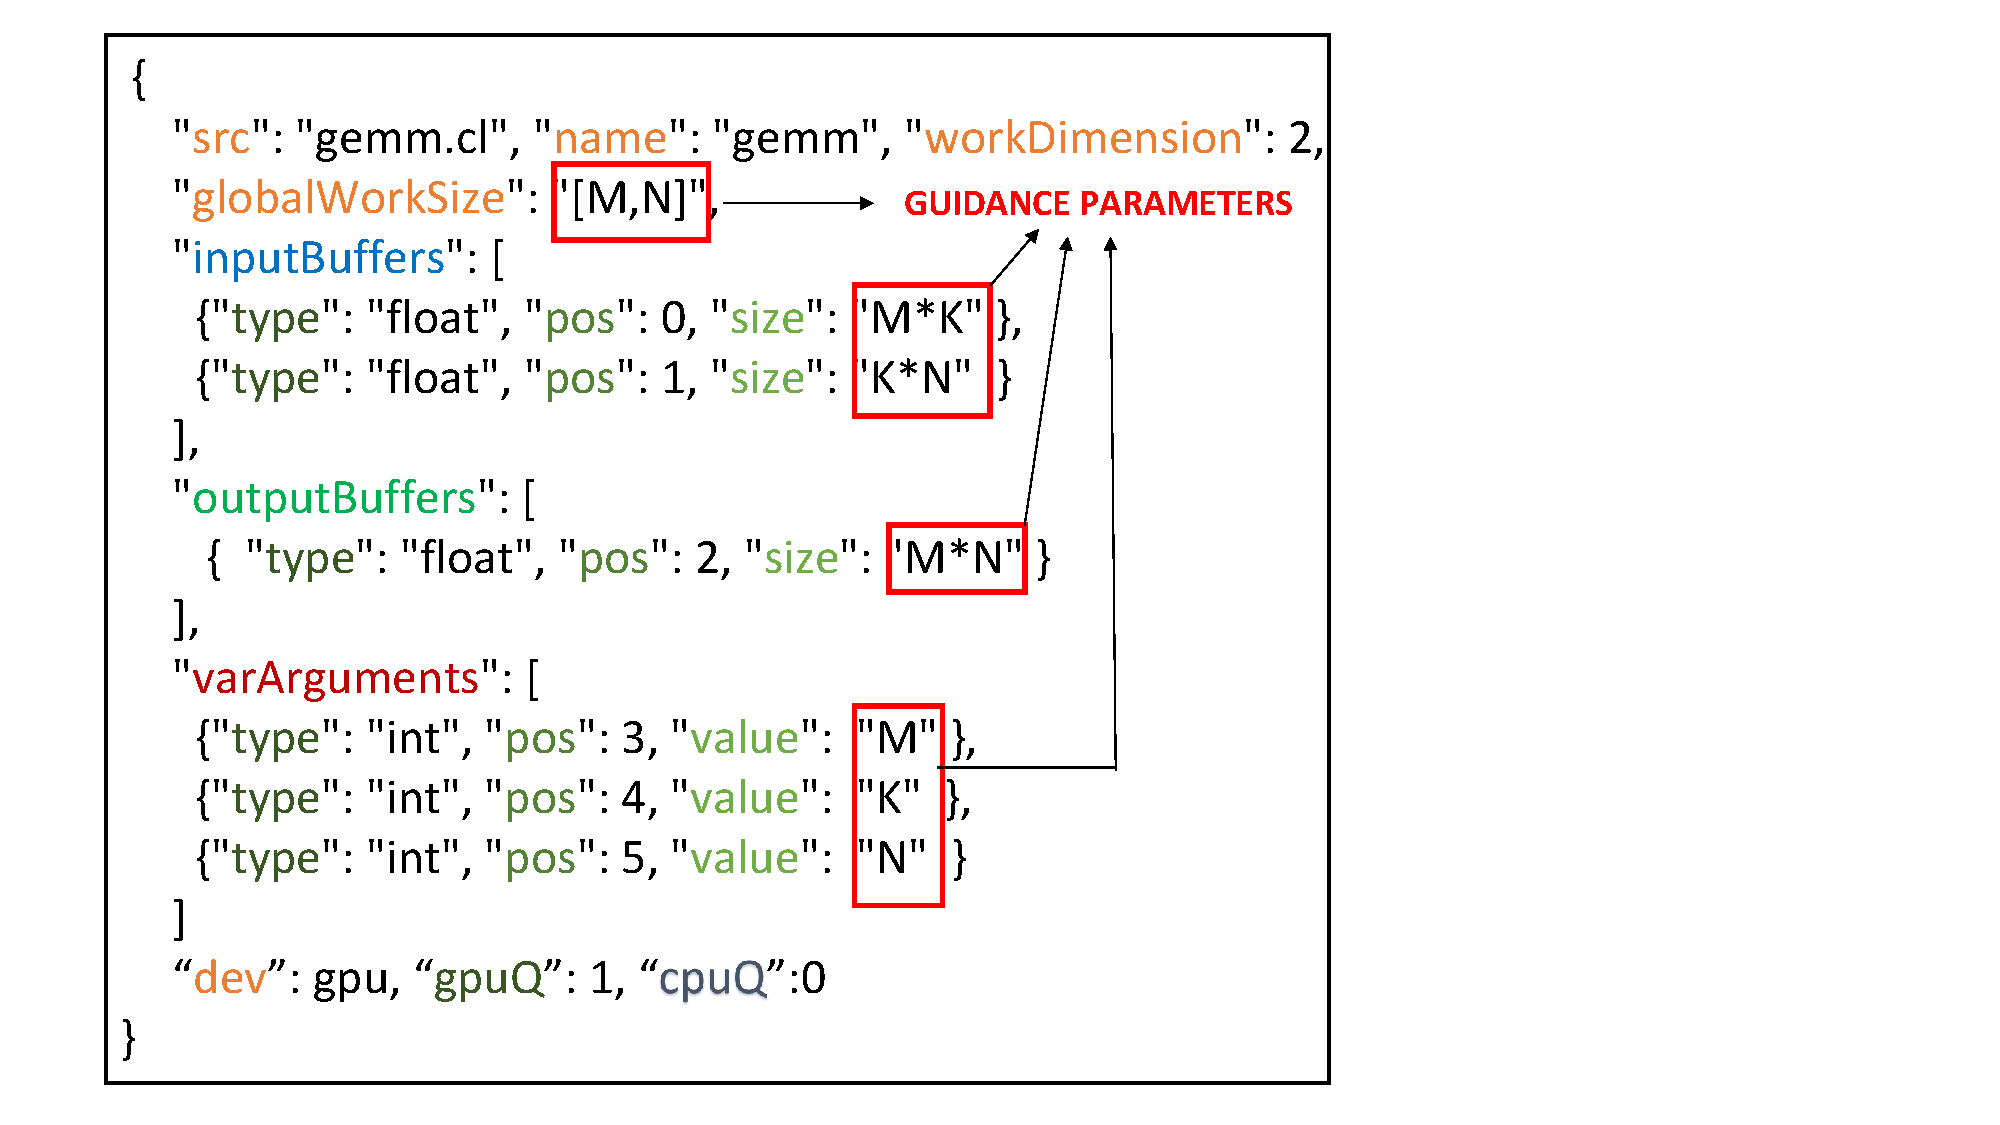
\includegraphics[scale=0.4]{Pictures/json_file.pdf}
		\caption{JSON File for Matrix Multiplication \label{fig:json}}
    \end{figure}
    
    The file comprises the following information.
	\begin{enumerate}
		\item \textbf{Kernel Information: } This includes i) the name of the OpenCL kernel function (which is {\tt gemm} in Fig. \ref{fig:json}), ii) the filepath of the required kernel source file, iii) the dimensionality of the kernel in {\tt workDimension} and iv) the total number of work items ({\tt globalWorkSize}) to be launched for this kernel. The variable {\tt globalWorkSize} is a three element list where each element refers to the number of work items along a particular dimension. As guidance parameters, the user can specify these elements either as compile time constants or using an generic expression containing symbolic variables. For the example JSON file, we have {\tt globalWorkSize = [M,N,1]}. The values of $M$ and $N$ can be configured  as command line parameters right before dispatching the kernel.  
		\item  \textbf{Buffer Information: }  The JSON file maintains information for three buffer lists - {\tt inputBuffers} reserved for input buffers, {\tt outputBuffers} reserved for output buffers and {\tt ioBuffers} reserved for buffers which are treated as both input and output  by the kernel. Each buffer belonging to any one of the lists is characterized by the tuple $\langle type, size ,pos \rangle$ where $type$ denotes the data type for each element in the buffer, $size$ denotes the total number of elements in the buffer, and $pos$ denotes the index position of the buffer argument in the actual function call of the kernel. For example, the input buffer passed as argument in the first position of the function call in Listing 1 has  $pos=0$. The user can configure the guidance parameter $size$ for each buffer either as a compile time constant or an expression of symbolic variables. For the example JSON file in Fig. \ref{fig:json}, the sizes of the buffers are the number of elements for each matrix. 
		\item \textbf{Kernel Arguments: } In the JSON file, each variable argument passed as an argument to the OpenCL function call is denoted by the tuple $\langle type, value, pos\rangle$  where $type$ denotes the type of the variable, $value$ represents the value contained in the variable and $pos$ represents the index position of the variable argument in the actual function call of the kernel. The user can configure the guidance parameter $value$  again either as a compile time constant or as a symbolic variable. In Fig. \ref{fig:json}, we have three variable arguments $M,N,K$ each depicting the size of one dimension of the matrices.
		\item \textbf{Device Information: } Finally, the $dev$ field indicates which device to be used. The fields $gpuQ$ and $cpuQ$ denote the number of command queues to be used for the GPU and the CPU devices respectively.
    \end{enumerate}
    
    \begin{figure}[ht]
		\centering
		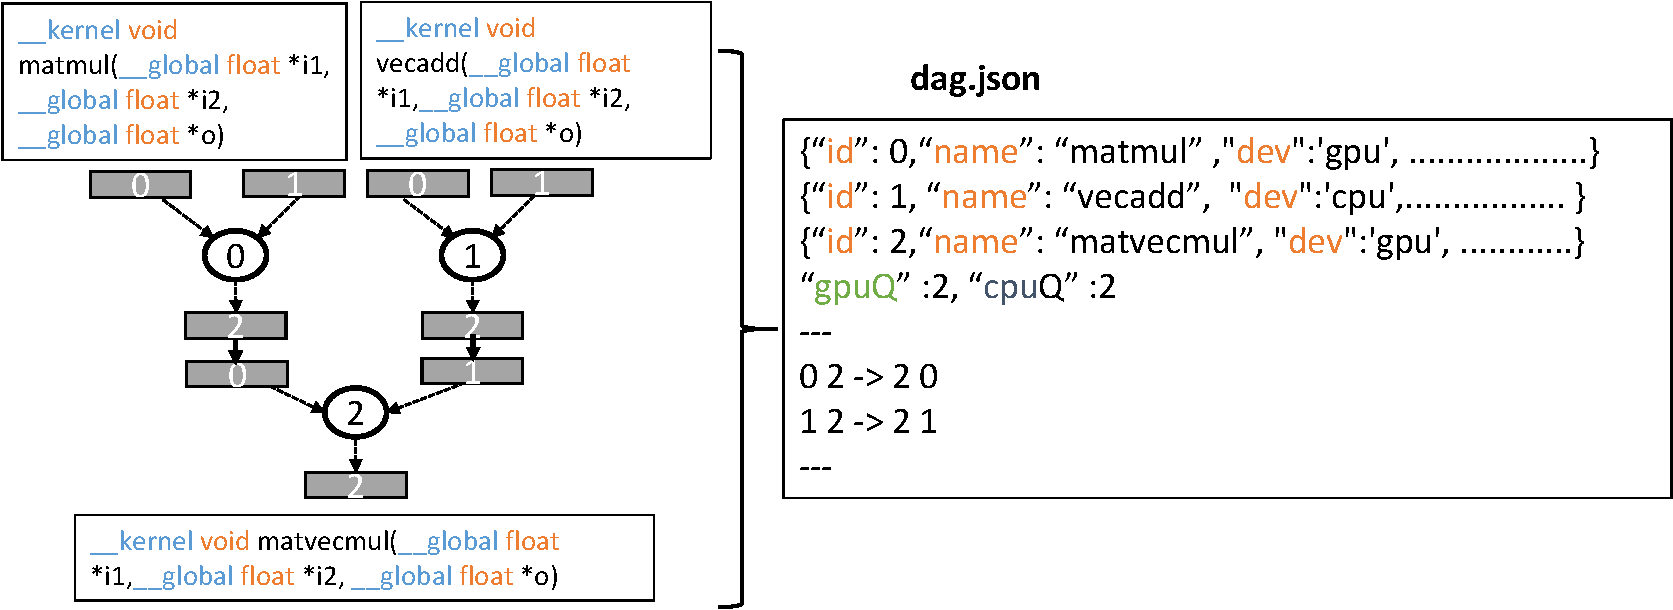
\includegraphics[scale=0.5]{Pictures/DAGJson.pdf}
		\caption{\small OpenCL DAG Specification\label{fig:OpenCLDAG}}
	\end{figure}
	\par \noindent In general a DAG of OpenCL kernels, can be specified as a single JSON file which contains the information regarding each kernel generated by running the compiler pass on each kernel. The user additionally has to specify information that captures the precedence constraints of the DAG. Unlike frameworks like SOCL, StarPU and MultiCL which requires implementing host-side implementations, our framework relies only on the DAG specification provided as a simple JSON file with configuration parameters of individual kernels and dependency information of the DAG.  
    \par Let us consider an example DAG comprising three kernels as depicted in Fig. \ref{fig:OpenCLDAG}. Each kernel now is designated by a unique identifier field called $id$. The kernel with id $0$ represents matrix multiplication kernel which takes as input two matrices of dimensions $M \times K$ and $K \times N$ and produces an output of dimension $M \times N$. The corresponding sizes of the input and output buffers are specified inside the JSON file of the kernel using these symbolic variables. The kernel with id $1$ represents a vector addition kernel which takes two vectors of size $N$ and produces one output vector of size $N$. The kernel with id $2$ represents  matrix-matrix multiplication kernel which takes as input an $M\times N$ matrix and $N\times 1$ vector and produces an $M \times 1$ vector. Again, the corresponding sizes of the input and output buffers for these kernels are specified in the individual JSON files of the kernels. The outputs of the kernels $1$ and $2$ are used by the kernel with id $2$. The dependency information for the same is specified as a set of edges of the form $k_i,b_r \rightarrow k_j,b_s$, where $k_i$,$k_j$ represent kernel ids that are dependent, $b_r$ is an output buffer of $k_i$ and $b_s$ is an input buffer of $k_j$ i.e. $(k_i,b_r) \in E_O$, $(b_s,k_j) \in E_I$ and $b_r,b_s \in E$. The ids for the buffers $b_r$ and $b_s$ are represented by their corresponding argument positions in the function call for the kernels. For example, if we consider $0,2 \rightarrow 2, 0$, the output buffer specified in argument 2 of kernel $0$ will be used as input buffer specified in argument 0 of kernel $2$. As guidance parameters, the user can specify the device preference for each kernel using the {\tt dev} field. In Fig. \ref{fig:json}, the kernels with ids 0 and 2 are mapped as a task component to the GPU device while kernel with id $1$ is mapped to the CPU device. The framework automatically takes care of setting up command queues specified in the fields $cpuQ$ and $gpuQ$ so as to maximally exploit concurrency using the scheduling engine which is discussed next.
    
	\section{Scheduling Backend}
	\subsection{Introduction}
	This section extensively uses the definitions (Definition \ref{def:task-component} onwards) outlined in Chapter \ref{Chapter3}. 
	An overview of the scheduling backend is depicted in Fig. \ref{fig:schedbackend}. 
	% We explain the working principle of the backend with the help of the procedure $schedule$ highlighted in Algorithm \ref{algo:dispatch} for scheduling. 
	% The input to $schedule$ is the application graph $G$ and the set of devices in the target platform $\mathcal{P}$. The procedure first parses the input specification and extracts the set of task components that are ready for dispatch (line 2).

    \begin{definition}
        \emph{We say a task component $T$ is \textbf{ready for dispatch} if for any kernel $k_i \in FRONT(T)$, i) there exists no predecessor or ii) all predecessors of $k_i$ have finished execution.}
	\end{definition}
	
	\begin{definition} \label{def:free_kernel}
		\emph{For a task component $T$ we define $\mathbf{T.free\_kernels}$ as a subset of kernels of T, such that $\forall k_{i} \in T.free\_kernels$, i) there exists no predecessor or ii) all predecessors of $k_i$ have been enqueued to a command queue of some device.}
	\end{definition}

	
	Note that in Definition \ref{def:free_kernel}, we do not require the predecessors of $k_i$ to have finished execution. Rather, we require them to just have been enqueued to any command queue. This distinction plays a key role in the functioning of the scheduler. 
	
	
	\subsection{The Two Scheduler Levels}
	PyschedCL's scheduler consists of two tiers. 
	\begin{itemize}
		\item \textbf{Coarse Grained Scheduler} - This component is a single threaded routine that is responsible for resource allocation (i.e. devices) to the task components. It maintains a data structure called the frontier queue $\mathcal{F}$, which is a list of task components that are ready to dispatch. It also maintains another data structure $\mathcal{A}$, which is a list of free devices. It uses the customisable {\tt select} routine to select a task component from $\mathcal{F}$ to dispatch and allocate resources to it. After the selection stage, it launches an instance of the \textbf{fine grained scheduler} on a new thread, which launches the kernels of the selected task component. The functioning of the coarse grained scheduler is defined in the {\tt schedule} procedure of Algorithm \ref{algo:dispatch}
		\item \textbf{Fine Grained Scheduler} - For a given task component $T$, the fine grained scheduler exhaustively enqueues all the kernels in $T.free\_kernels$. It's input is the tuple $(T,Q)$, where Q is the list of command queues associated with the device allocated by the Coarse Grained Scheduler. To maximise fine grained concurrency, it matches kernels in $T.free\_kernels$ with command queues in $Q$ in a round robin fashion. It also sets up the dependencies between execute events as shown in Figure \ref{fig:finecoarse} to ensure correctness. After enqueuing a kernel it also updates the $free\_kernels$ data structure of the task components of it's children according to Definition \ref{def:free_kernel}. It's functioning is defined in the {\tt enq} procedure of Algorithm \ref{algo:dispatch}.
	\end{itemize}

	\subsection{Scheduling Algorithm}
    \begin{algorithm}[H]
		
		\caption{Scheduling in PySchedCL\label{algo:dispatch}}
		\textbf{Input: } $G$ - an OpenCL Application DAG, $\mathcal{P}$ - set of target platform devices
		\begin{algorithmic}[1]
			\Procedure{schedule}{$G$,$\mathcal{P}$}
			\State $\mathcal{F} \leftarrow get\_free\_task\_components(G)$ , $\mathcal{A} \leftarrow \mathcal{P}$
			\While{all kernels of $G$ not finished}
			\While{$\mathcal{A}$ contains a device and $\mathcal{F}$ is not empty}
			\State $T,Q \leftarrow select(\mathcal{F},\mathcal{A})$
			\State $enq(T,Q)$
			% \State $set\_callbacks(T,Q)$
			% \State $dispatch(T,Q)$
			\EndWhile
			\EndWhile
			\EndProcedure

			\Function{enq}{$T$,$\mathcal{Q}$} 
			
			\While{$T.free\_kernels$ is not empty}		
			\State $k \leftarrow T.free\_kernels.pop()$
			\State $q \leftarrow pop(\mathcal{Q})$
			\State $enqueue(k,q)$
			\State $set\_dependencies(k,\mathcal{Q})$
			\State $push(q,\mathcal{Q})$
			\If{$k \in END(T)$}
				\State $set\_callback(k)$
			\EndIf
			\For{$k_i \in k.children$}
				\If{$k_i$ satisfies Definition \ref{def:free_kernel}}
					\State Add $k_i$ to $T_i.free\_kernels$ where $T_i$ is the task component of $k_i$.
					\If{$T_i \neq T$ and $T_i \notin \mathcal{F}$}
						\State Add $T_i$ to $\mathcal{F}$
					\EndIf
				\EndIf
			\EndFor
			\EndWhile
			\EndFunction
		\end{algorithmic}
	\end{algorithm}

    

	 Algorithm \ref{algo:dispatch} provides the pseudocode of the scheduler. The functioning of the coarse grained scheduler is defined by the procedure {\tt schedule}. The $select$ routine is used to select a task component $T$ and an empty command queue data structure $\mathcal{Q}$ for an available device belonging to $\mathcal{A}$. The number of command queues to be used in $\mathcal{Q}$ for a device $d$ is specified as a guidance parameter by the user in the specification file. 
	\begin{figure}[ht]
		\centering
		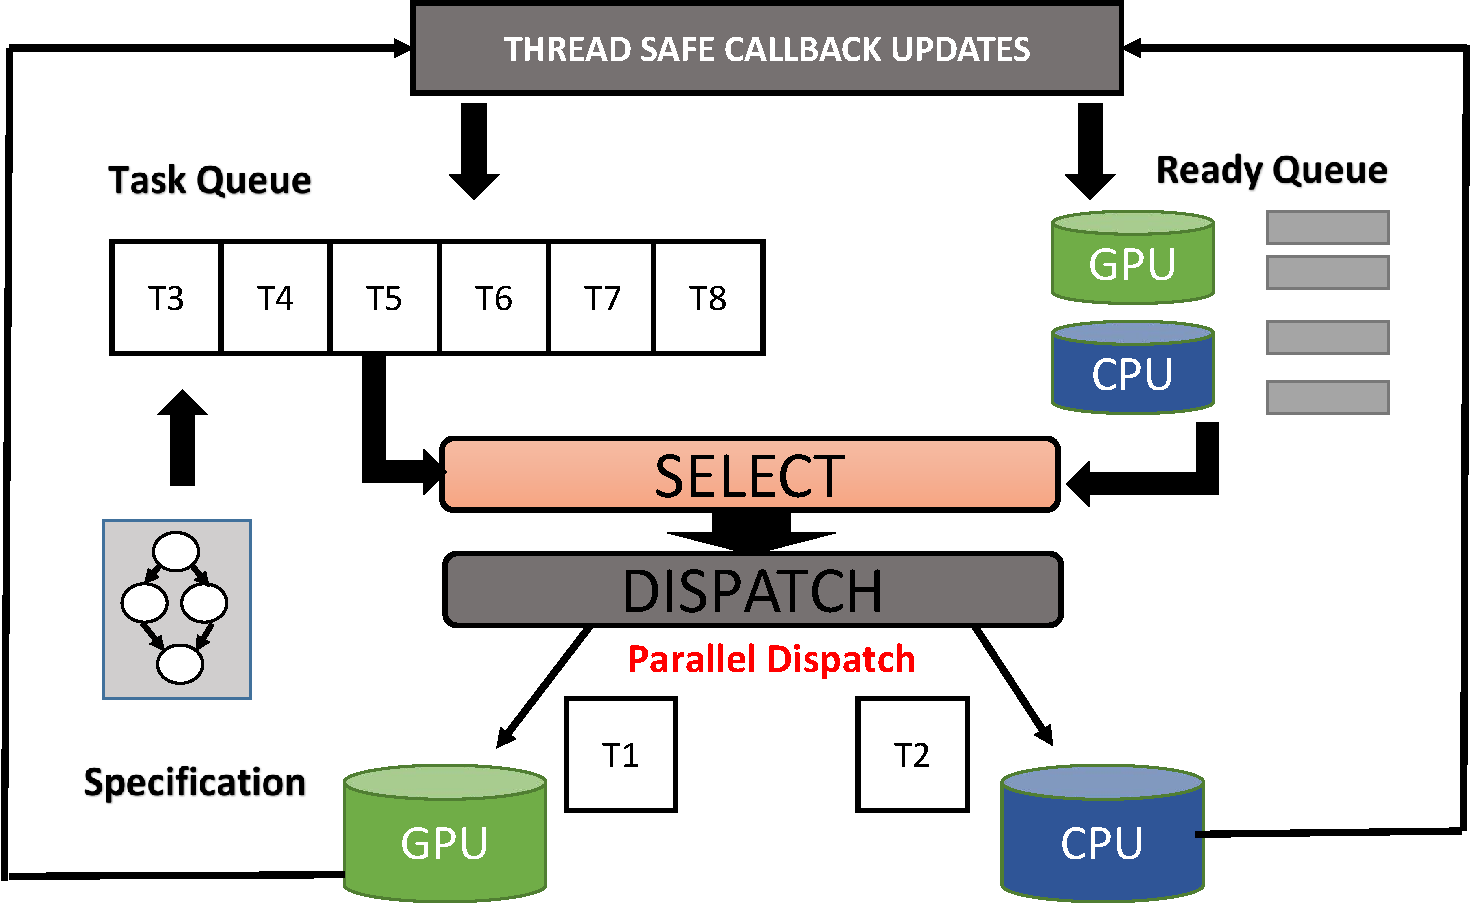
\includegraphics[scale=0.35]{Pictures/SchedulingEngine.pdf}
		\caption{\small Command Queue Setup\label{fig:schedbackend}}
    \end{figure}
    
    Given any task component $T$ and the list of allocated command queues by the coarse grained scheduler - $\mathcal{Q}$ for a device $d$, the $enq$ procedure is used to populate  $\mathcal{Q}$ with operations pertaining to kernels belonging to $T$ as illustrated in Figure \ref{fig:finecoarse}.  We explain the working principle of the function with the help of an illustrative example depicted in Fig. \ref{fig:dispatch} where we map a task component comprising 5 kernels to a GPU device using a total of 3 command queues. 
	\begin{figure}[ht]
		\centering
		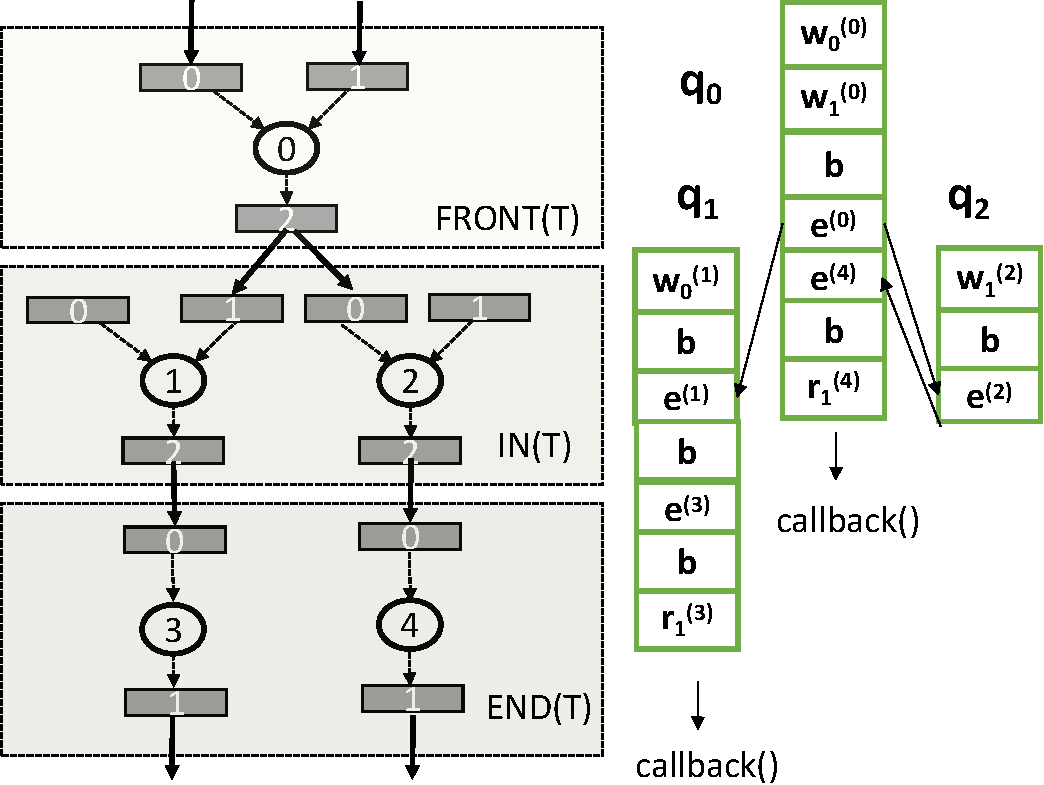
\includegraphics[scale=0.45]{Pictures/TaskObject.pdf}
		\caption{\small Command Queue Setup\label{fig:dispatch}}
	\end{figure}
	 A free kernel $k$ is first selected from $T.free\_kernels$ (line 9) and a queue $q$ is selected from $\mathcal{Q}$ using $pop(\mathcal{Q})$(line 10). The list of command queues in $\mathcal{Q}$ is maintained as a circular queue by the framework. The required read, write and ndrange operations of kernel $k$ are next pushed to command queue $q \in V_Q$. In Fig. \ref{fig:dispatch}, we observe for kernel $0$, two write operations $w_0^{(0)},w_1^{(0)}$ being pushed first to $q_0$ followed by a barrier, and an ndrange operation $e^{0}$. Since kernel $0 \in FRONT(T)$, the writes correspond to the two inter edges. The $enq$ function next sets up dependencies between relevant operations i.e. $E_Q$ of $\mathcal{Q}$ using $set\_dependencies()$ (line 15). For kernel $0$, we have no dependencies to set. Once this is done, the command queue $q$ is pushed back to $V_Q$ of $\mathcal{Q}$ for future use if required. The free kernels list of all the task components of successors of $k$ is updated now (lines 17-18), and these task components are added to $\mathcal{F}$ if they are not present there (lines 19-20). From Fig. \ref{fig:dispatch}, we observe that for kernels $1$ and $2$ belonging to $IN(T)$, only the isloated write operations $w_0^{(1)}$ and  $w_1^{(2)}$ are added to $q_1$ and $q_2$ respectively. This is followed by the barrier operations and the respective ndrange operations $e^{1}$ and $e^{2}$. The $set\_dependencies()$ function sets up dependencies between $e^{0}$, $e^{1}$ and $e^{0}$, $e^{2}$. Furthermore, since $w_0^{1}$ and $w_1^{2}$ are mapped to different command queues $q_1$ and $q_2$, they can execute in parallel while operations in $q_0$ are executing. After using queue $q2$, queues $q0$ and $q1$ are again used   for kernels with ids $3$ and $4$ respectively. Since they belong to $END(T)$, only the execute operations followed by barrier and read operations are pushed to the respective command queues. We note for coarse-grained scheduling decisions,  all relevant operations will be enqueued to one single command queue in $\mathcal{Q}$.
	\par Once the command queue data structure $\mathcal{Q}$ has been populated, the {\tt dispatch} function is called which is responsible for enqueuing the command queues with read,write and ndrange operations as specified in $\mathcal{Q}$. Once this call is made, the associated command queues are locked i.e. they cannot be used by other task components that are ready for dispatch.  Once all relevant {\tt clEnqueue } OpenCL API calls are made, the {\tt clFlush()} function is called once per command queue in $\mathcal{Q}$ to ensure that the commands are submitted to the device. We further note, if multiple tasks components are ready for dispatch, then multiple {dispatch} calls are initiated in parallel, i.e. separate threads are spawned which are responsible for setting up the command queues for each device.
	
	\par The $set\_callback$ function (line 15) is used to set up callback functions  for the read operations corresponding to every write from output buffer $b_i$ to $b_j$ such that $(k_r,b_i) \in E_O$ and $k_r \in END(T)$ and $b_i,b_j$ is an intra-edge. The callbacks are set using {\tt clSetEventCallback()} function for the read operations via events as discussed earlier. Since the successor kernels of $k_r$ belong to a different task component mapped to a different device, the buffer $b_i$ needs to get copied back to the host. For kernels getting mapped to CPU devices sharing the same memory space as that of the host, the callbacks are associated with the ndrange operations of each kernel $k_i$, since buffer reads and writes in this context are redundant.
    \par The callbacks are thread-safe i.e. they perform atomic updates to the shared data structures $\mathcal{F}$ and $\mathcal{A}$. As depicted in Fig. \ref{fig:schedbackend}, each callback function is responsible for two distinct operations - i) adding successor task components which are ready for dispatch to the task queue and ii) releasing the command queues which were locked, once all kernels of the the task component finish execution. Since, it may be possible that multiple callbacks can execute simultaneously as a consequence of multiple kernels belonging to the task component $T$ finishing at the same time, it is imperative that the callback functions execute in a thread-safe manner to ensure correctness in updating the respective queues. 
    
    \par The procedure $schedule$ highlights a generic procedure for scheduling algorithms in our framework. As discussed before, the end user can override the select routine and experiment with different scheduling policies. We implement two dynamic coarse-grained scheduling algorithms and one static fine-grained scheduling algorithm and present experimental results for the same, continuing with our  motivational example from Section \ref{sec:motivation}.





    